\subsection{Diseño de usuario}

\subsubsection{Análisis del proceso propuesto}

En la Figura \ref{fig:proceso-propuesto} se presenta el proceso propuesto para el envió de alertas de emergencia con
ubicación en tiempo real, en donde:

\begin{enumerate}
    \item Si el usuario no se encuentra registrado en el sistema:
          \begin{enumerate}
              \item El usuario se registra en el sistema.
              \item El usuario inicia sesión en el sistema.
          \end{enumerate}
    \item El usuario ingresa miembros a su grupo familiar.
    \item El usuario selecciona un tipo de incidente.
          % \item El usuario envía la alerta de emergencia presionando el bot��������n de pánico durante 3 segundos.
    \item El usuario envía la alerta de emergencia presionando el botón de pánico durante 3 segundos.
    \item Se envía una notificación a los miembros del grupo familiar del usuario y los policías dentro de la zona de emergencia junto con la ubicación en tiempo real.
    \item El Ecu 911 recibe la alerta de emergencia y la asigna a la entidad correspondiente.
    \item La emergencia es atendida.
\end{enumerate}

\begin{figure}[H]
    \centering
    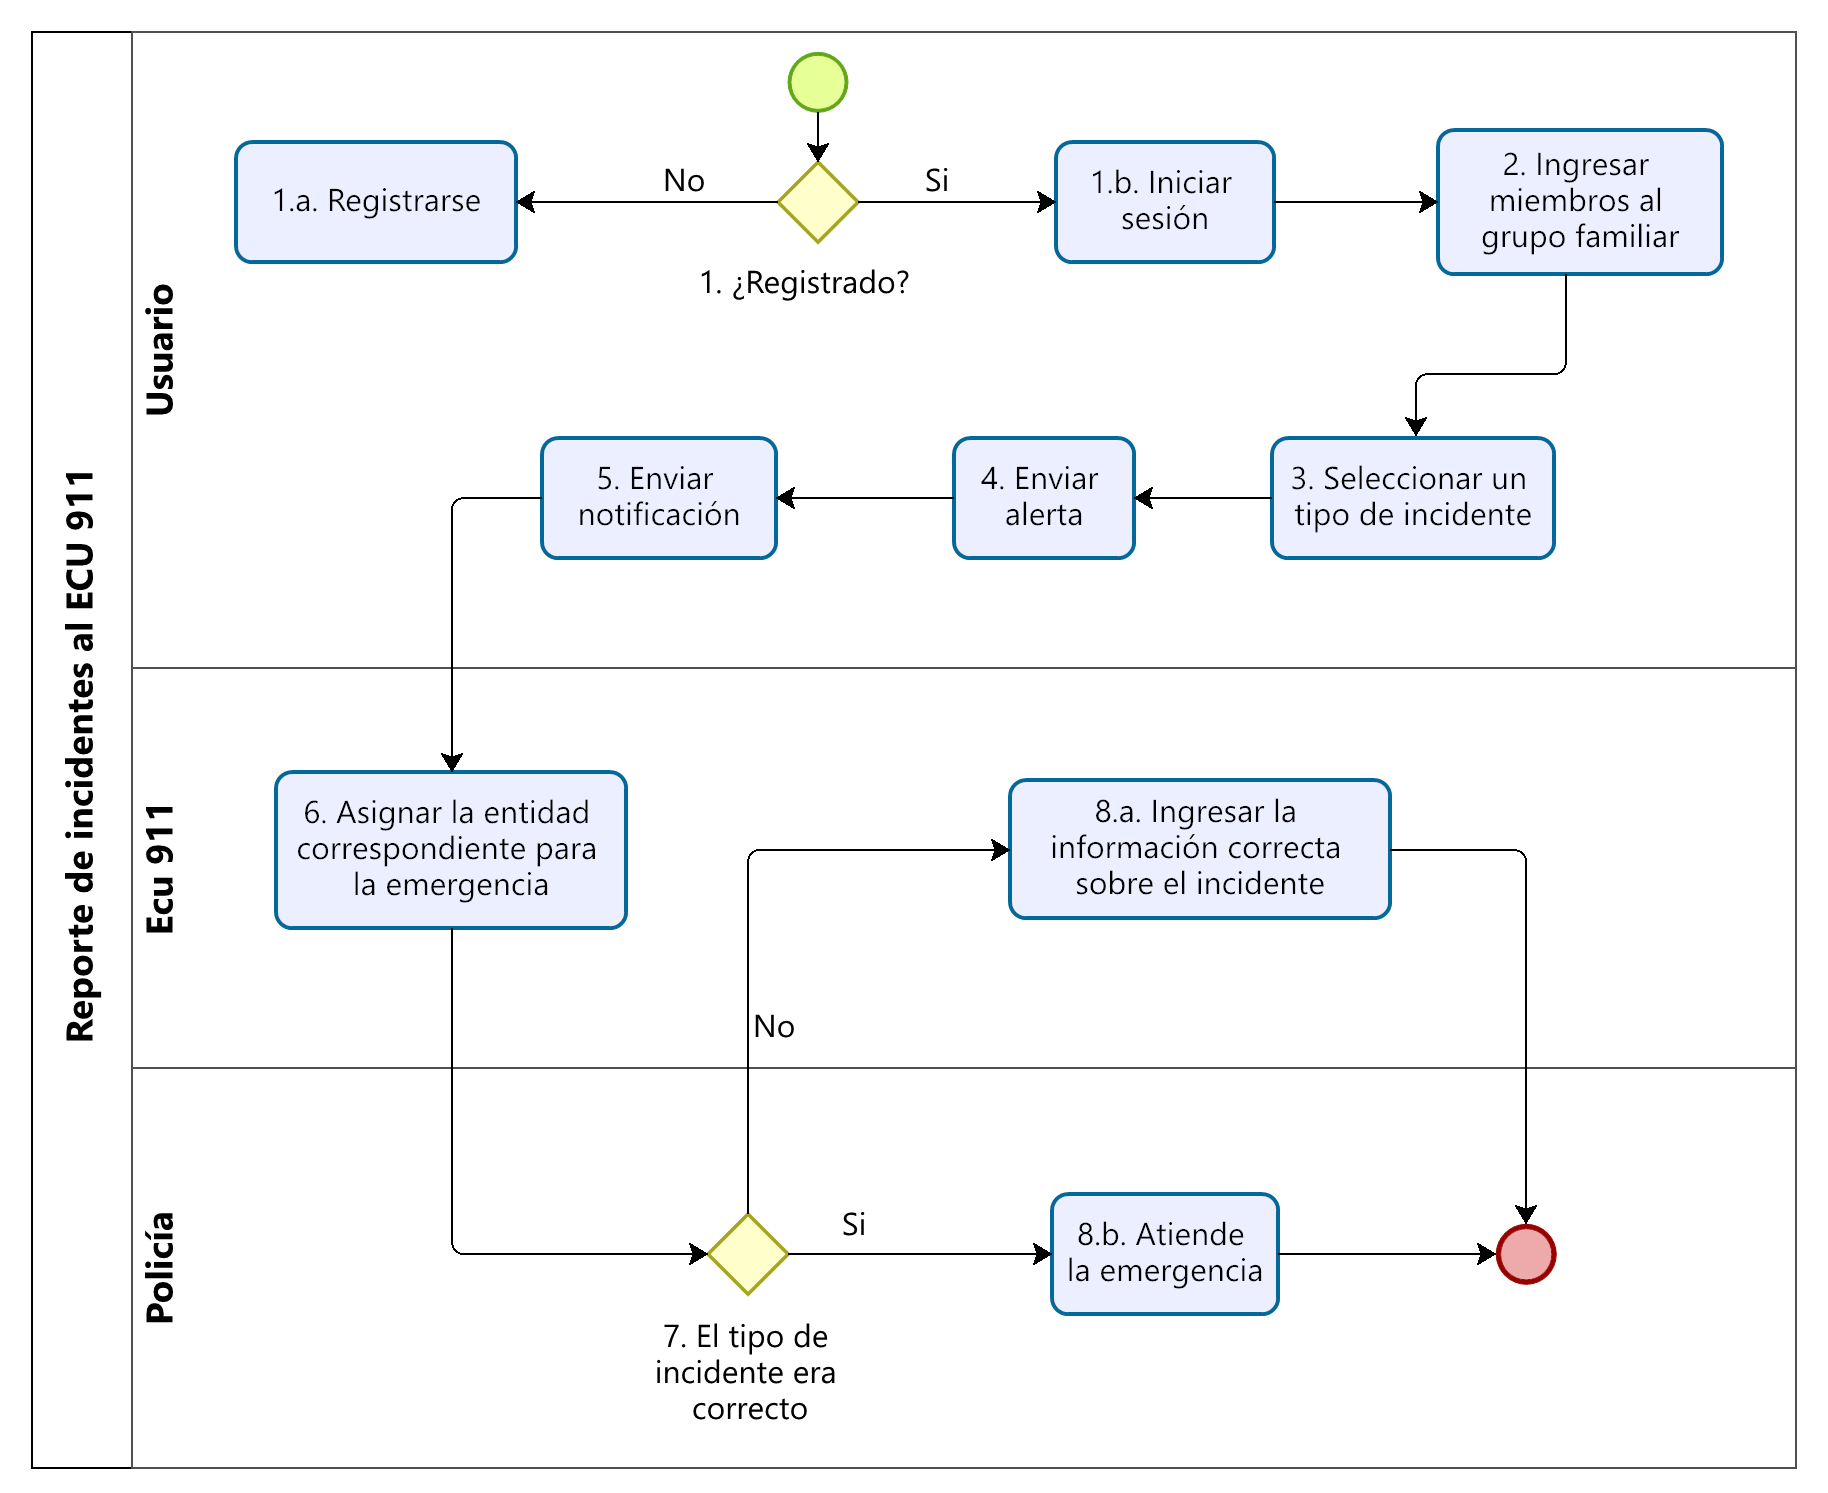
\includegraphics[width=0.8\textwidth]{chapters/III-resultados-y-discusion/resources/images/proceso-propuesto.png}
    \caption{Proceso propuesto de reporte de incidentes al ECU 911.}
    \label{fig:proceso-propuesto}
\end{figure}

\subsubsection{Arquitectura}

El desarrollo del sistema se estructuró en 2 partes fundamentales: la API y La interfaz de usuario, tanto web como móvil.
La interfaz de usuario en el sistema web permite a los administradores gestionar la información de los usuarios y los incidentes
ademas de visualizar la ubicación en tiempo real de los incidentes en un mapa. La interfaz de usuario en el sistema móvil
permite gestionar grupos familiares, enviar alertas de emergencia y visualizar la ubicación en tiempo real de los incidentes de sus
miembros del grupo familiar. El API se encuentra alojada en un servidor web y se encarga de gestionar la conexión entre la base de
datos, los servicios de almacenamiento de información, el servicio de hosting de imágenes, el servicio de web socket y las interfaces
de usuario.

\begin{figure}[H]
    \centering
    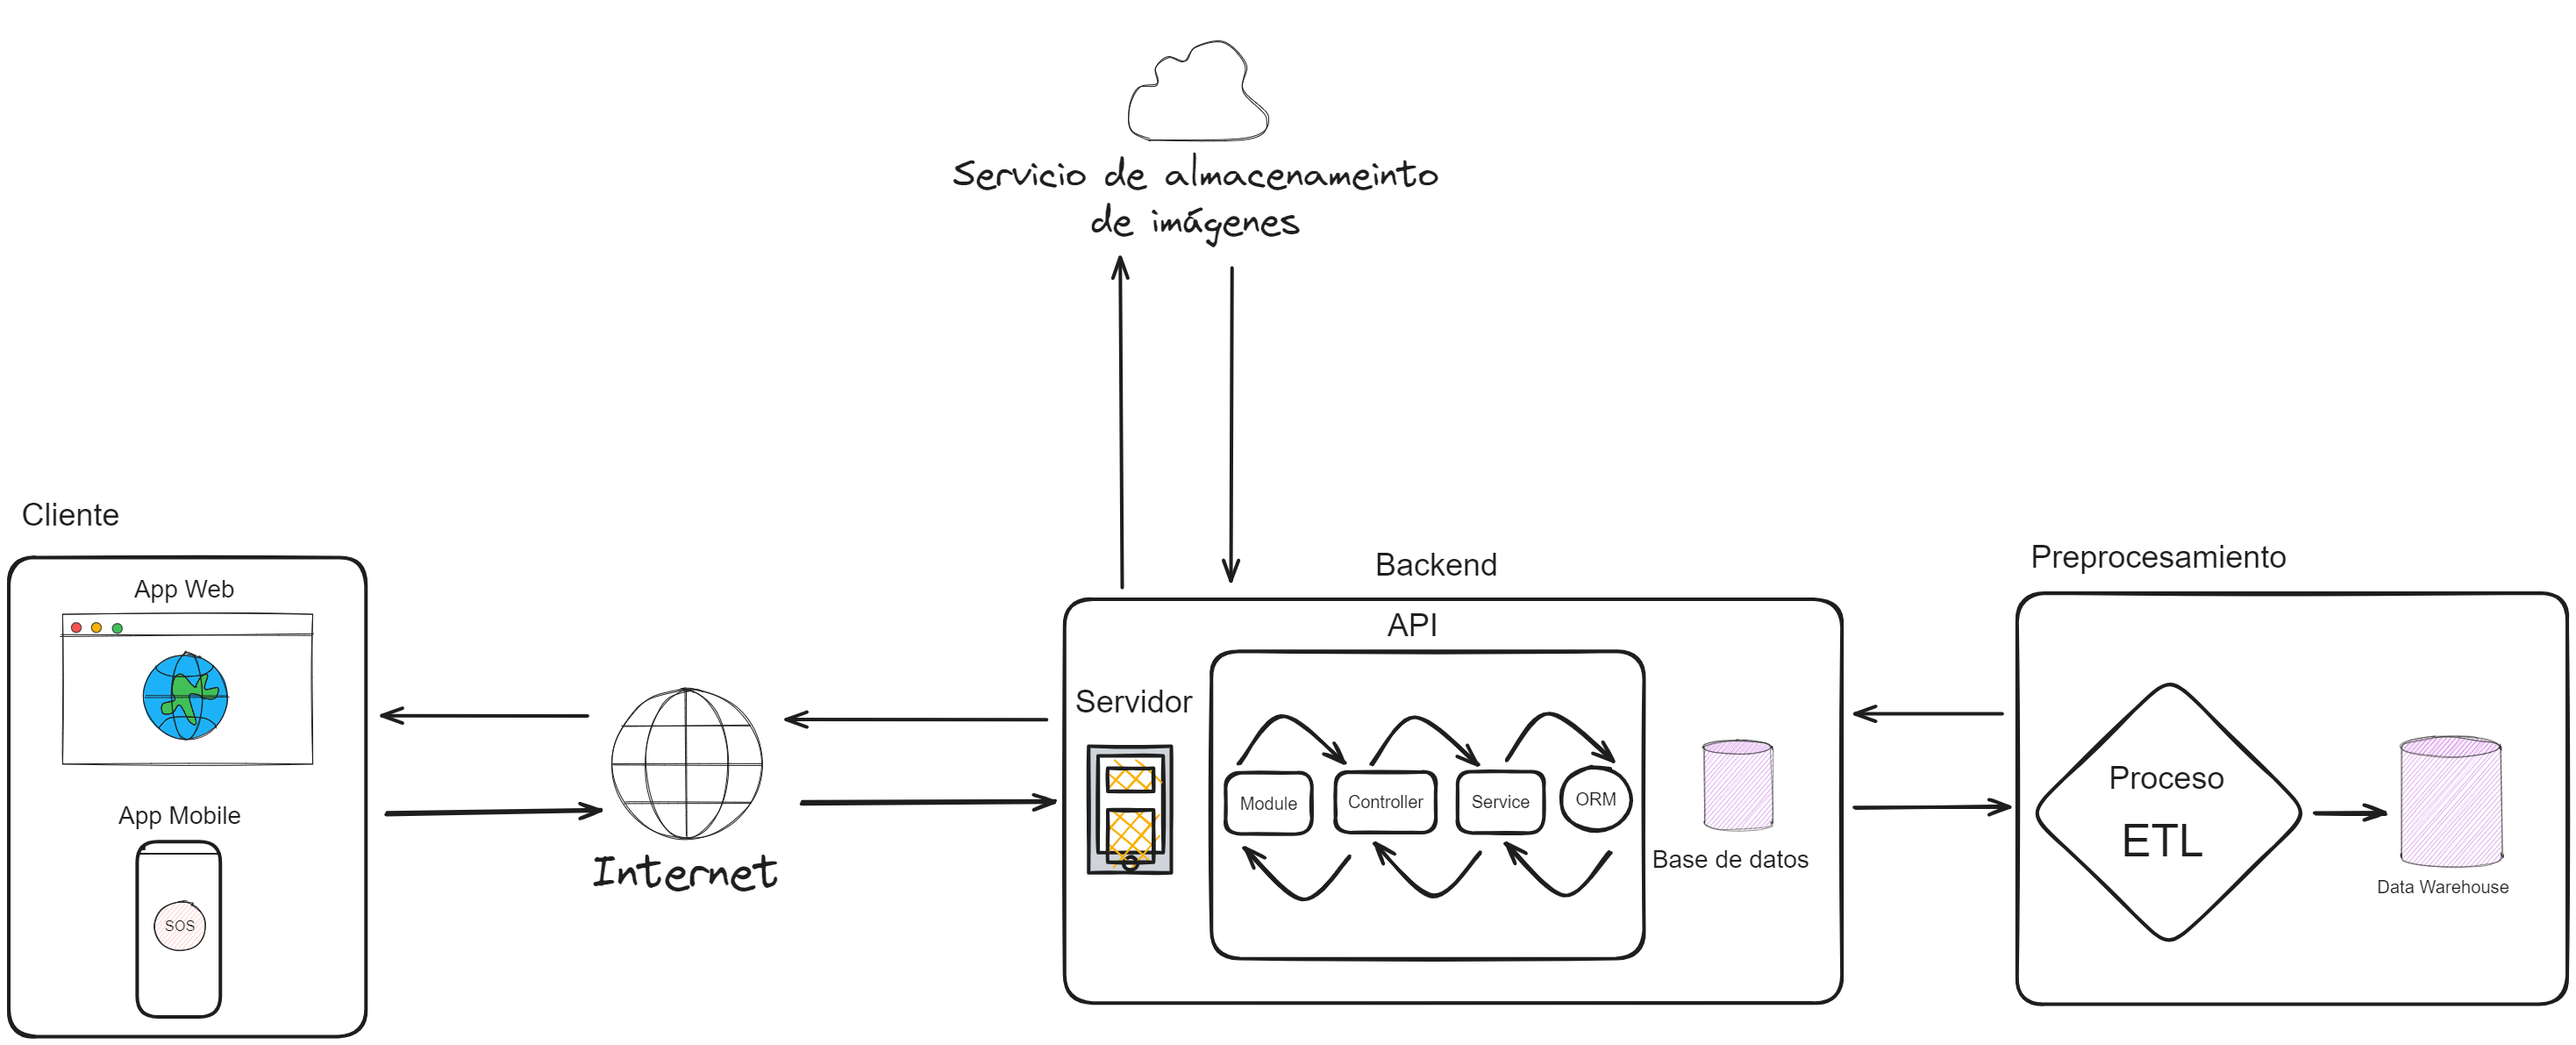
\includegraphics[width=1.1\textwidth]{chapters/III-resultados-y-discusion/resources/images/arquitectura.png}
    \caption{Arquitectura del sistema}
    \label{fig:arquitectura}
\end{figure}


\subsubsection{Prototipado}

En esta etapa de la metodología, se desarrollaron prototipos con el objetivo de identificar y resolver problemas de diseño y funcionalidad.
Esto permite detectar posibles fallos o áreas de mejora antes de la fase de construcción de la aplicación, optimizando así el proceso de
desarrollo y asegurando que el producto final sea más robusto y alineado con los objetivos del proyecto.

El prototipado para el sistema se divide en dos partes: el prototipo de la interfaz de usuario web y el prototipo de la interfaz de usuario móvil.

\subsubsection{Prototipo de la interfaz de usuario web}

En la Figura \ref{fig:prototipo-inicio-sesion-web} se presenta el prototipo de la interfaz de usuario web, donde se muestra la pantalla de inicio de sesión,
el cual se realiza mediante correo y contraseña.

\begin{figure}[H]
    \centering
    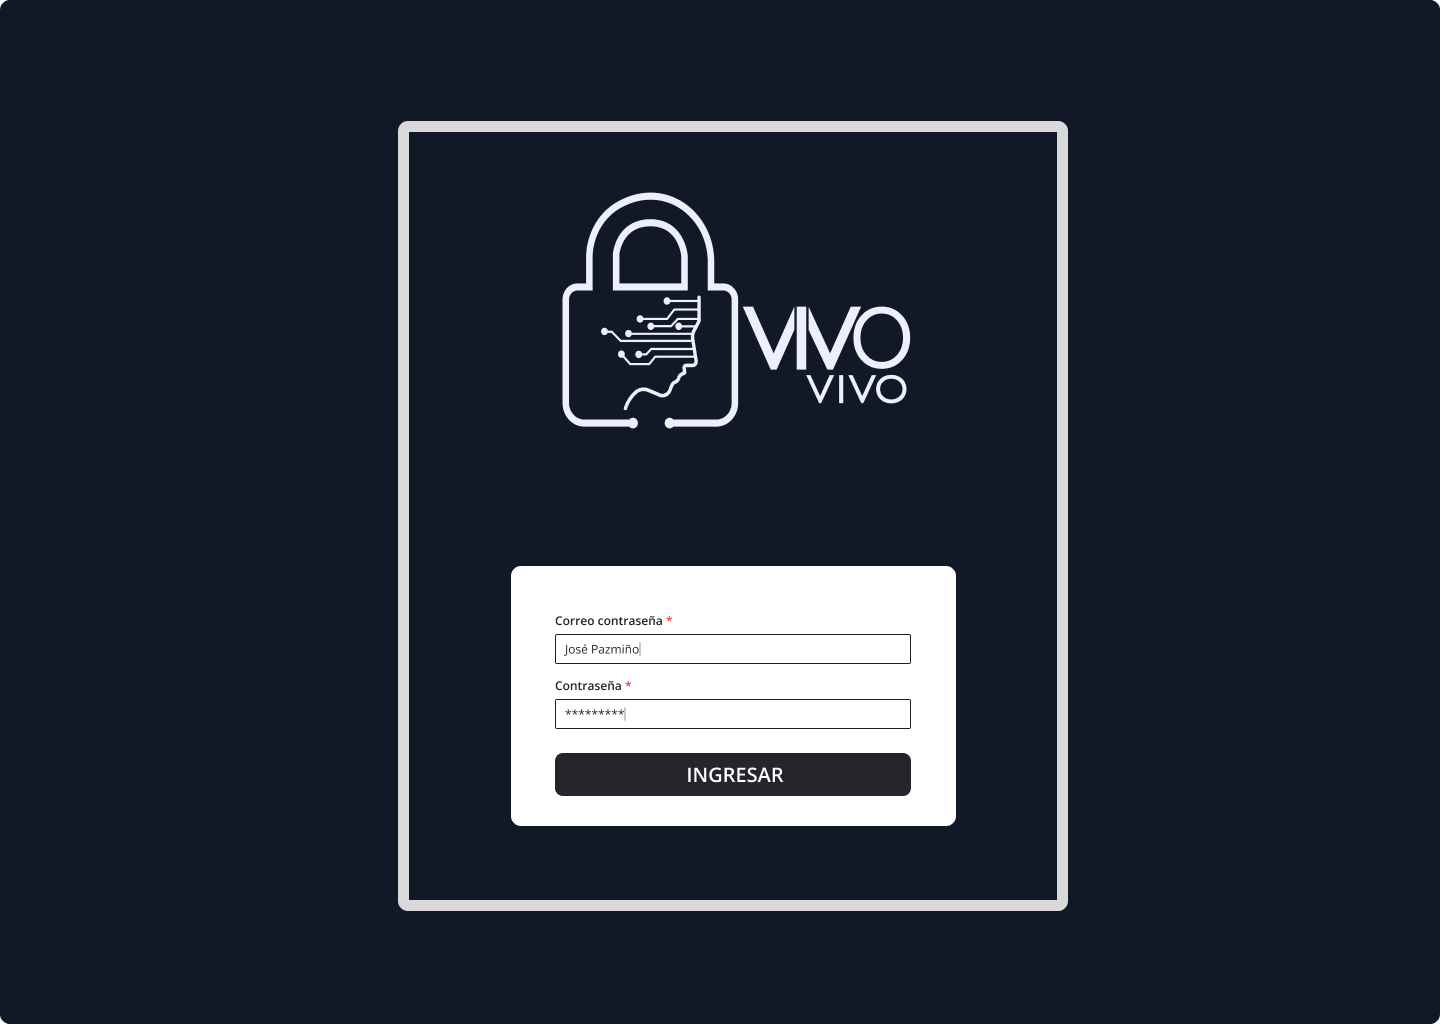
\includegraphics[width=0.6\textwidth]{chapters/III-resultados-y-discusion/resources/images/prototipo-inicio-sesion-web.png}
    \caption{Prototipo de la interfaz de usuario web: Inicio de sesión.}
    \label{fig:prototipo-inicio-sesion-web}
\end{figure}

En la Figura \ref{fig:prototipo-layout-web} se presenta el prototipo de la interfaz de usuario web, donde se muestra el layout de la aplicación web junto
con el menú de navegación y el menú de opciones

\begin{figure}[H]
    \centering
    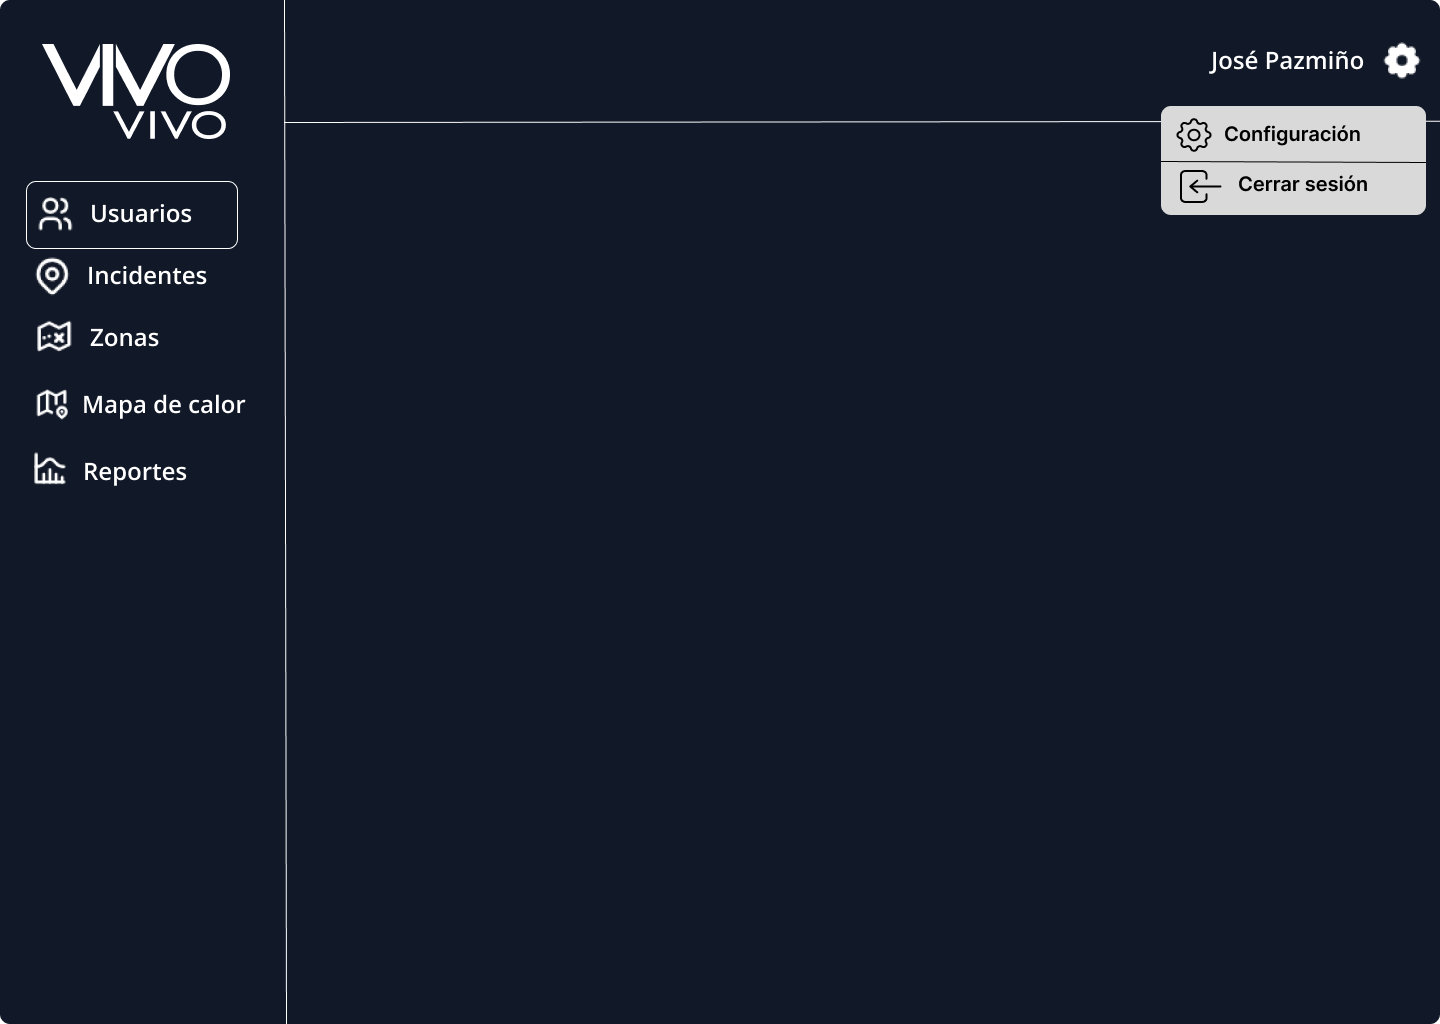
\includegraphics[width=0.6\textwidth]{chapters/III-resultados-y-discusion/resources/images/prototipo-layout-web.png}
    \caption{Prototipo de la interfaz de usuario web: Layout.}
    \label{fig:prototipo-layout-web}
\end{figure}

La gestión de la información en el sistema web se realiza a través de una tabla de entradas, la cual permite al usuario administrador crear, visualizar,
editar y eliminar los registros, así como también aplicar filtros de búsqueda, como se muestra en la Figura \ref{fig:prototipo-tabla-entradas-web}.

\begin{figure}[H]
    \centering
    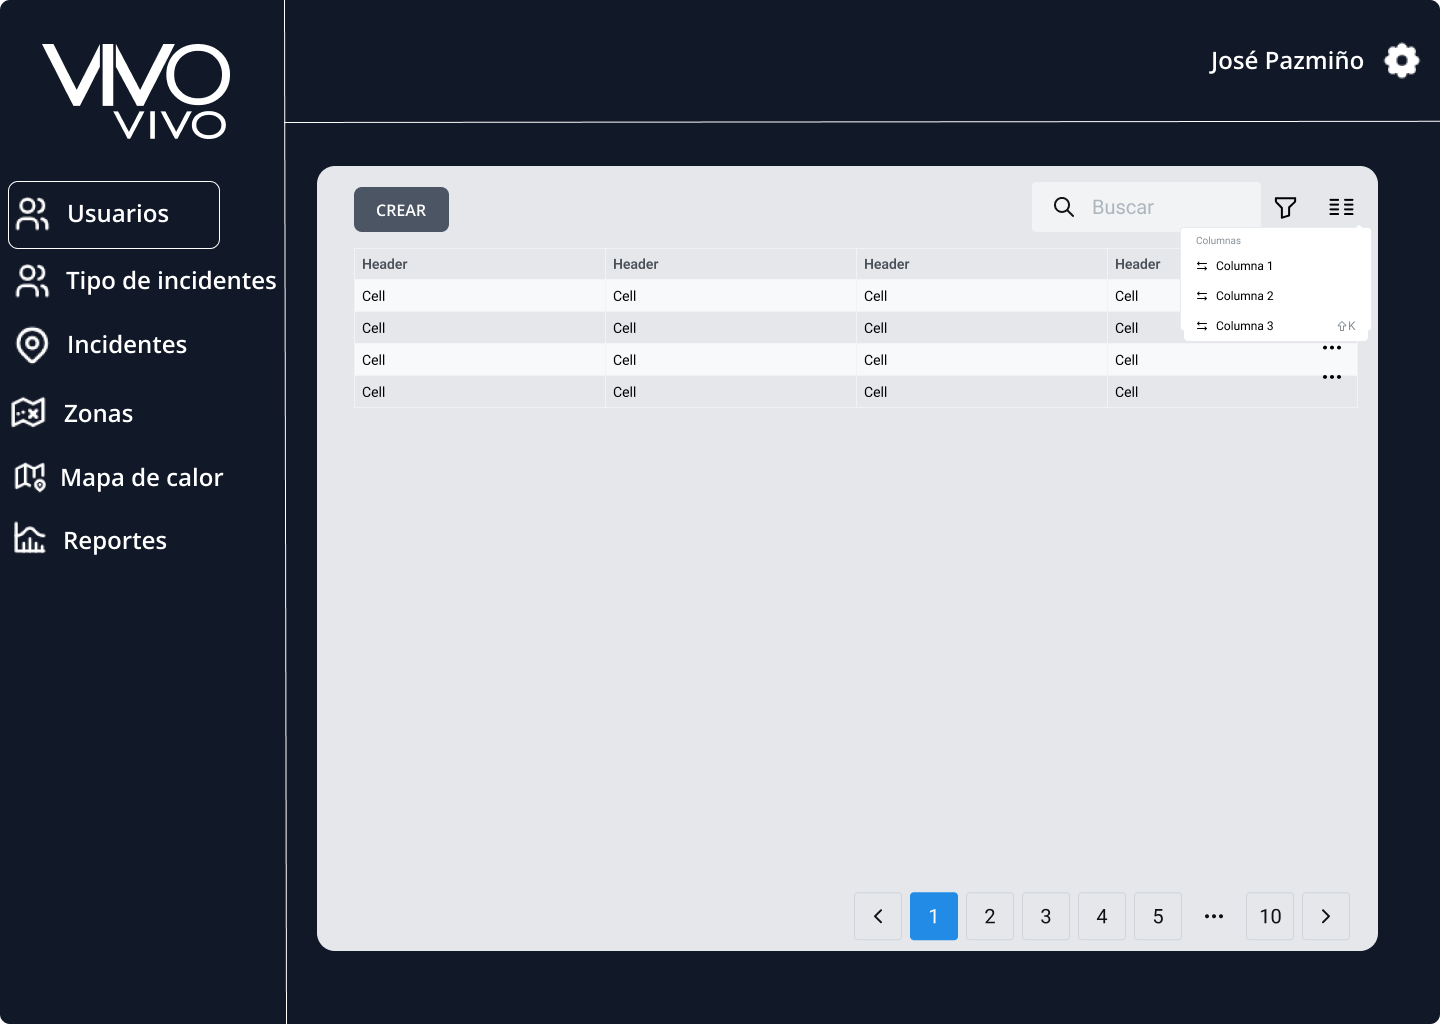
\includegraphics[width=0.6\textwidth]{chapters/III-resultados-y-discusion/resources/images/prototipo-tabla-entradas-web.png}
    \caption{Prototipo de la interfaz de usuario web: Tabla de entradas.}
    \label{fig:prototipo-tabla-entradas-web}
\end{figure}

En la Figura \ref{fig:prototipo-menu-tabla-entradas-web} se muestra el menú de opciones de la tabla de entradas, el cual permite al usuario administrador
realizar acciones como editar y eliminar registros. Al eliminar un registro, se muestra un mensaje de confirmación para ejecutar la acción, como se puede
observar en la Figura \ref{fig:prototipo-mensaje-eliminar-web}

\begin{figure}[H]
    \centering
    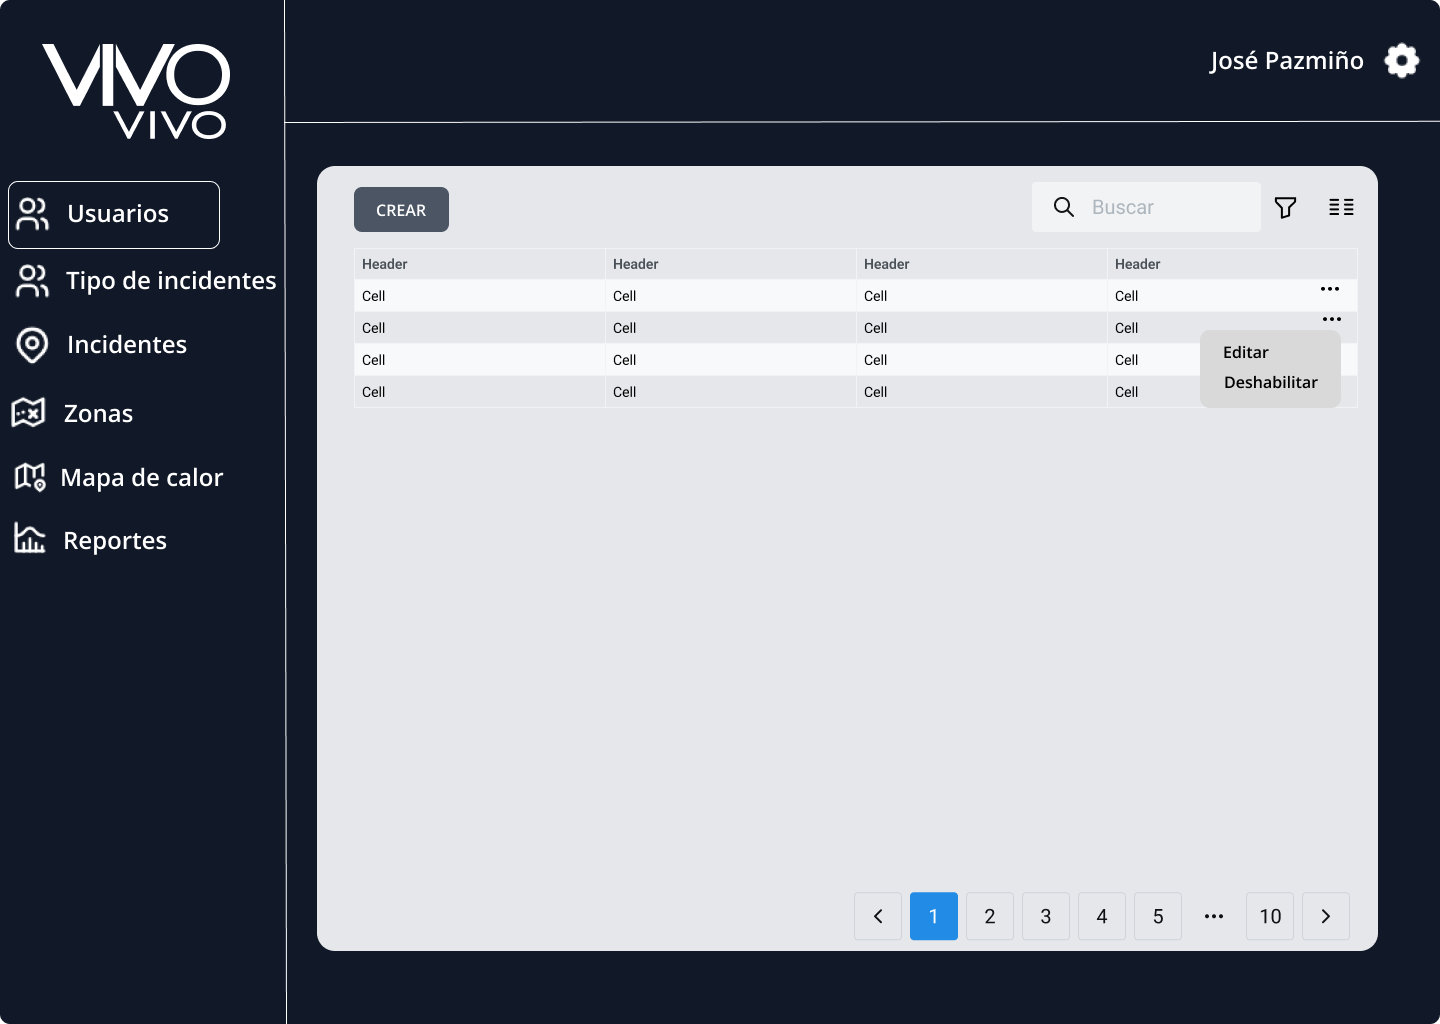
\includegraphics[width=0.6\textwidth]{chapters/III-resultados-y-discusion/resources/images/prototipo-menu-tabla-entradas-web.png}
    \caption{Prototipo de la interfaz de usuario web: Menú de opciones de la tabla de entradas.}
    \label{fig:prototipo-menu-tabla-entradas-web}
\end{figure}

\begin{figure}[H]
    \centering
    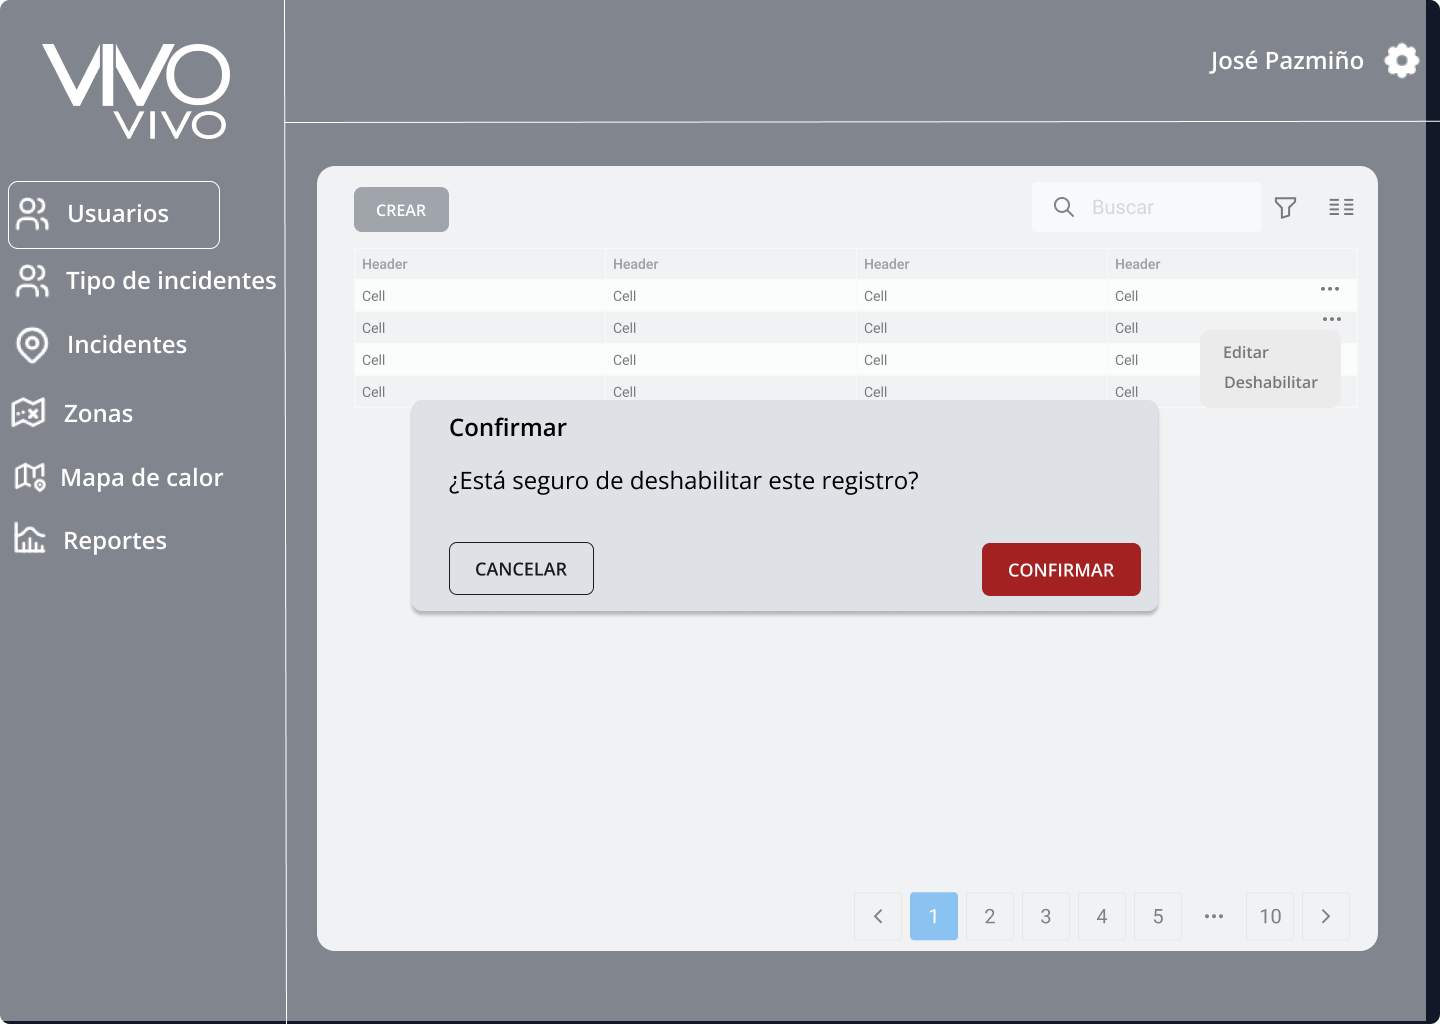
\includegraphics[width=0.6\textwidth]{chapters/III-resultados-y-discusion/resources/images/prototipo-mensaje-eliminar-web.png}
    \caption{Prototipo de la interfaz de usuario web: Mensaje de confirmación para eliminar un registro.}
    \label{fig:prototipo-mensaje-eliminar-web}
\end{figure}

Para la gestión de usuarios en el sistema web, la informaci��n de dichos usuarios se visualizará en una tabla, como se puede observar en la Figura
\ref{fig:prototipo-tabla-usuarios-web}. Se propone un formulario de registro en el cual el usuario administrador puede ingresar la información
necesaria para crear un nuevo usuario, así como actualizar la información de un usuario existente y eliminar un usuario, como se muestra en la Figura
\ref{fig:prototipo-formulario-usuario-web}.

\begin{figure}[H]
    \centering
    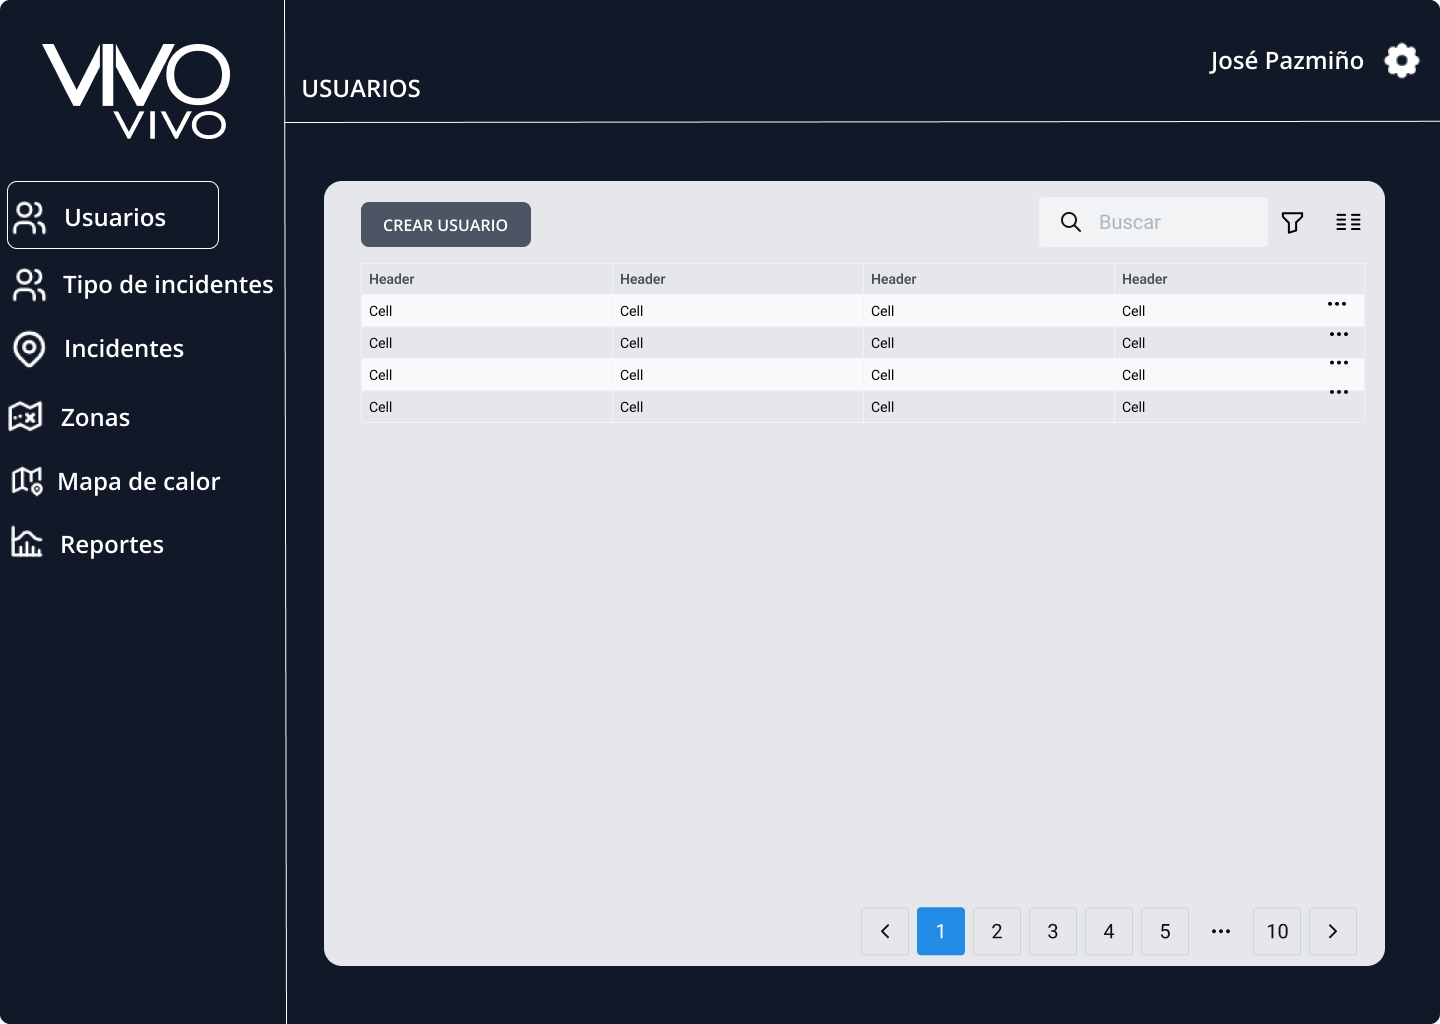
\includegraphics[width=0.6\textwidth]{chapters/III-resultados-y-discusion/resources/images/prototipo-tabla-usuarios-web.png}
    \caption{Prototipo de la interfaz de usuario web: Tabla de usuarios.}
    \label{fig:prototipo-tabla-usuarios-web}
\end{figure}

\begin{figure}[H]
    \centering
    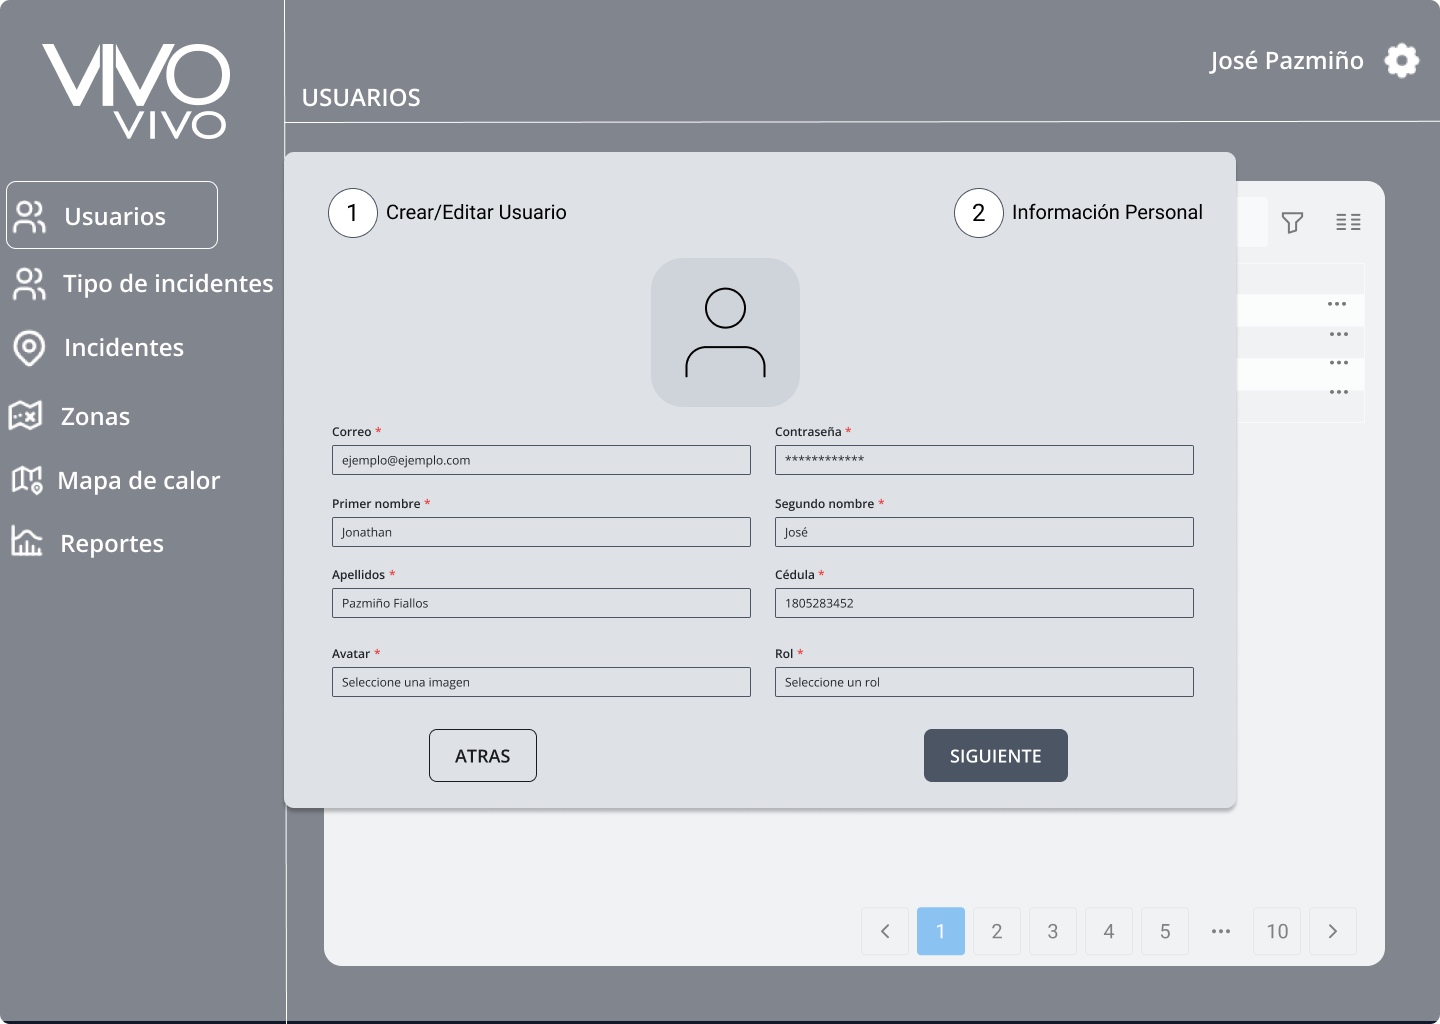
\includegraphics[width=0.6\textwidth]{chapters/III-resultados-y-discusion/resources/images/prototipo-formulario-usuario-web.png}
    \caption{Prototipo de la interfaz de usuario web: Formulario de usuario.}
    \label{fig:prototipo-formulario-usuario-web}
\end{figure}

Para la visualización de la información de los tipos de incidentes en el sistema web, se desarrolló una tabla de entradas, como se muestra en la Figura
\ref{fig:prototipo-tabla-tipos-incidentes-web}. Se propone un formulario de registro en el cual el usuario administrador puede ingresar la información
necesaria para crear un nuevo tipo de incidente, así como actualizar la información de un tipo de incidente existente y eliminar un tipo de incidente,
como se muestra en la Figura \ref{fig:prototipo-formulario-tipo-incidente-web}.

\begin{figure}[H]
    \centering
    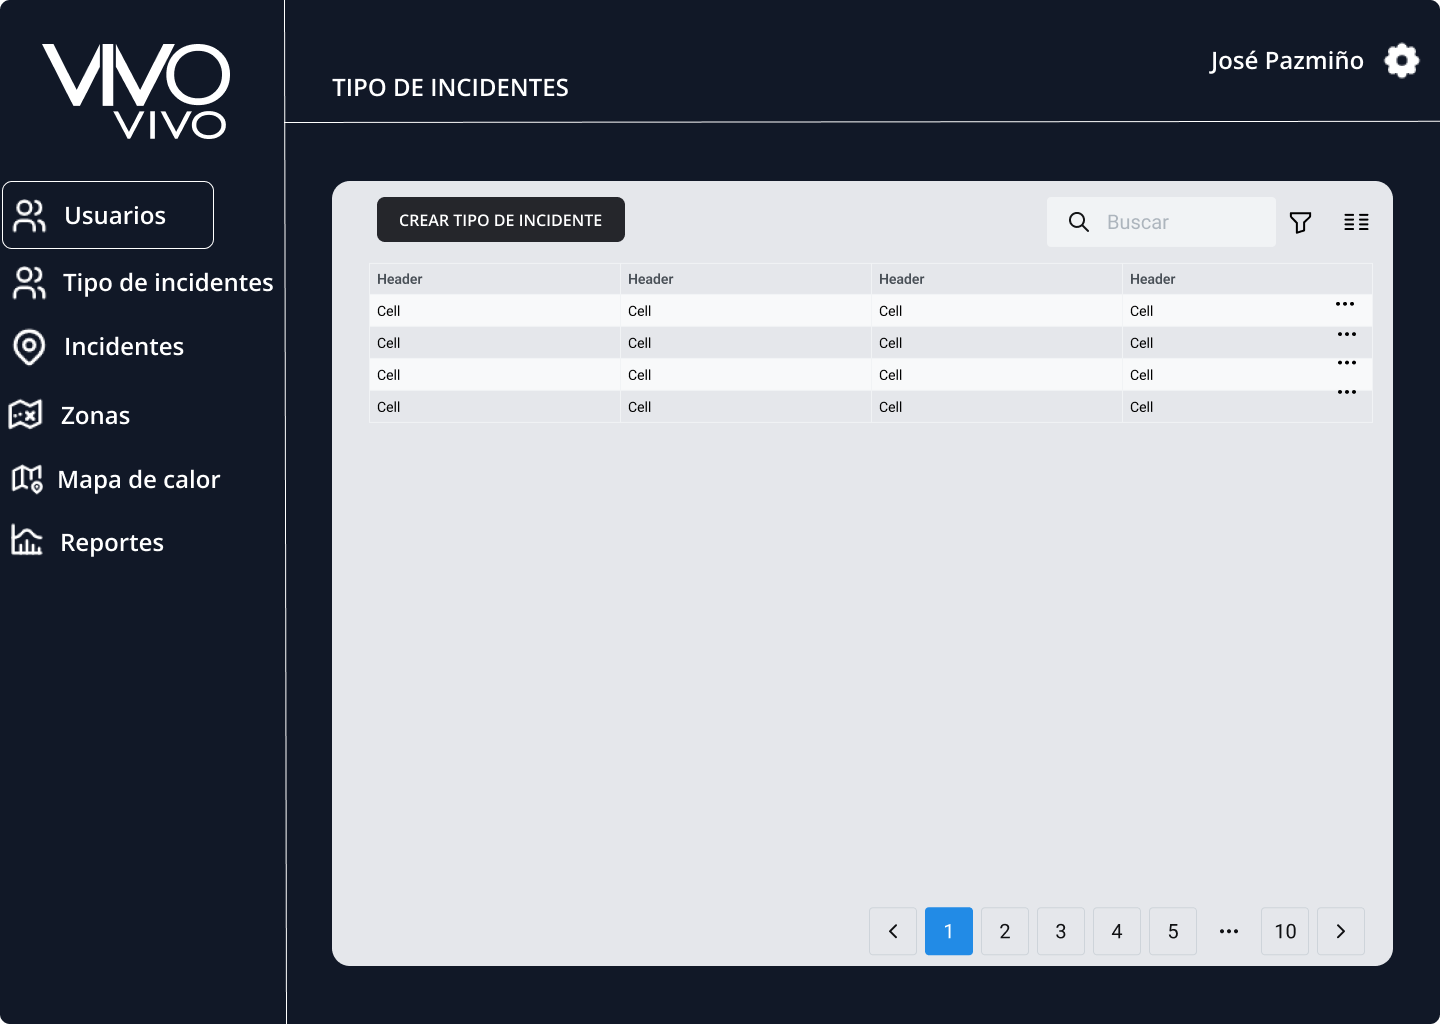
\includegraphics[width=0.6\textwidth]{chapters/III-resultados-y-discusion/resources/images/prototipo-tabla-tipos-incidentes-web.png}
    \caption{Prototipo de la interfaz de usuario web: Tabla de tipos de incidentes.}
    \label{fig:prototipo-tabla-tipos-incidentes-web}
\end{figure}

\begin{figure}[H]
    \centering
    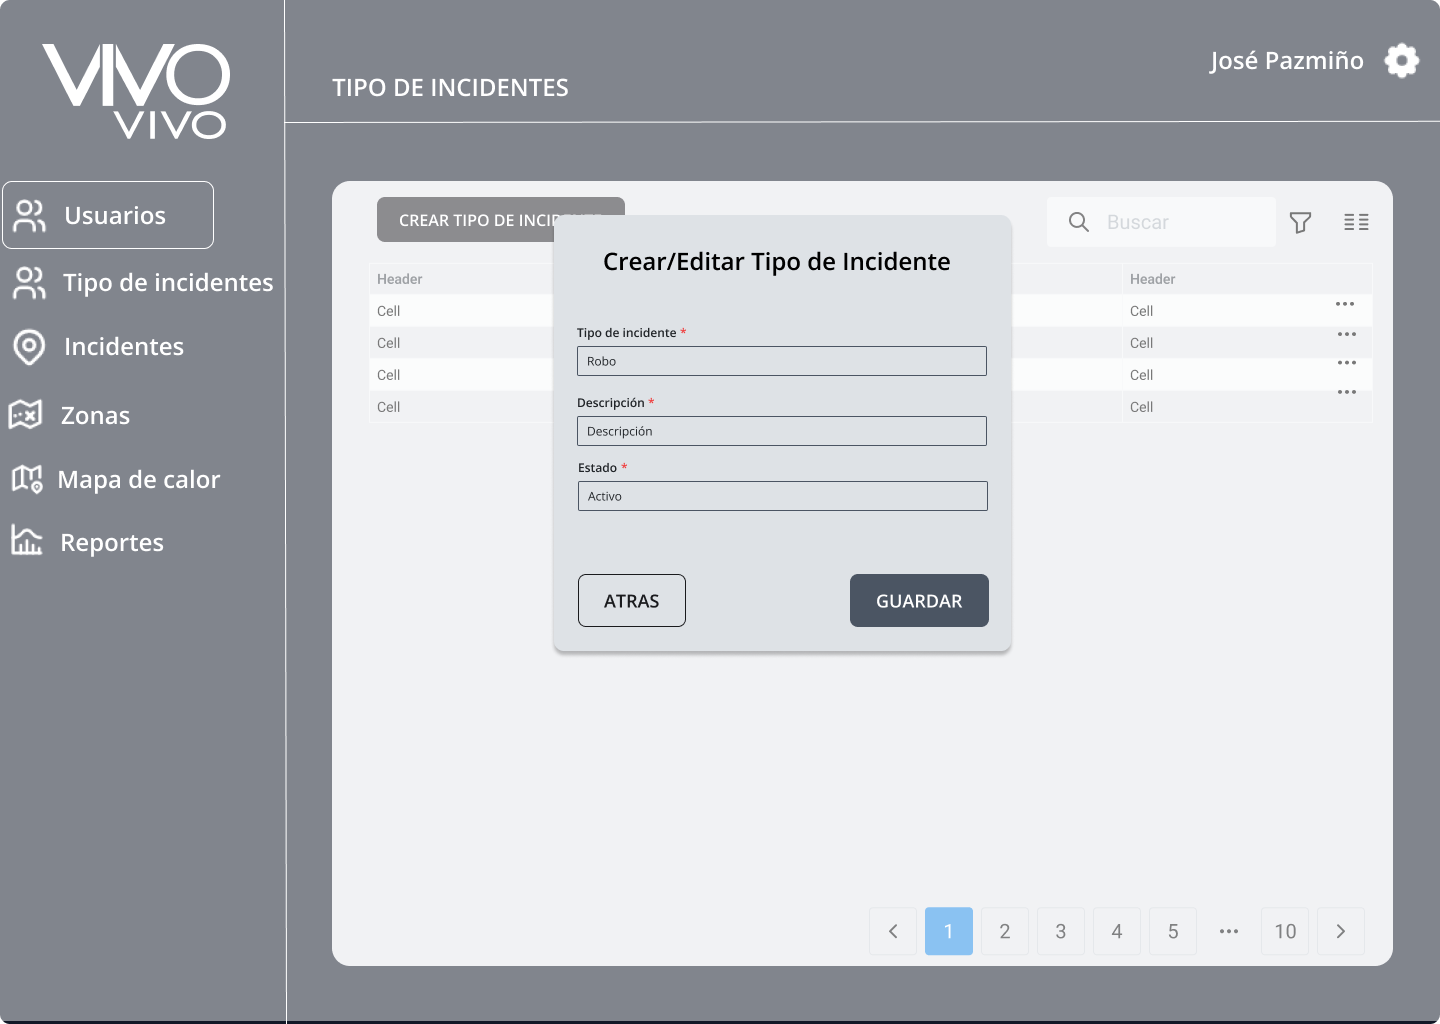
\includegraphics[width=0.6\textwidth]{chapters/III-resultados-y-discusion/resources/images/prototipo-formulario-tipo-incidente-web.png}
    \caption{Prototipo de la interfaz de usuario web: Formulario de tipo de incidente.}
    \label{fig:prototipo-formulario-tipo-incidente-web}
\end{figure}

En la Figura \ref{fig:prototipo-mapa-zonas-de-vigilancia-web} se muestra la pantalla de zonas de vigilancia, la cual permite al usuario administrador
visualizar las zonas de vigilancia mediante polígonos en un mapa interactivo.

\begin{figure}[H]
    \centering
    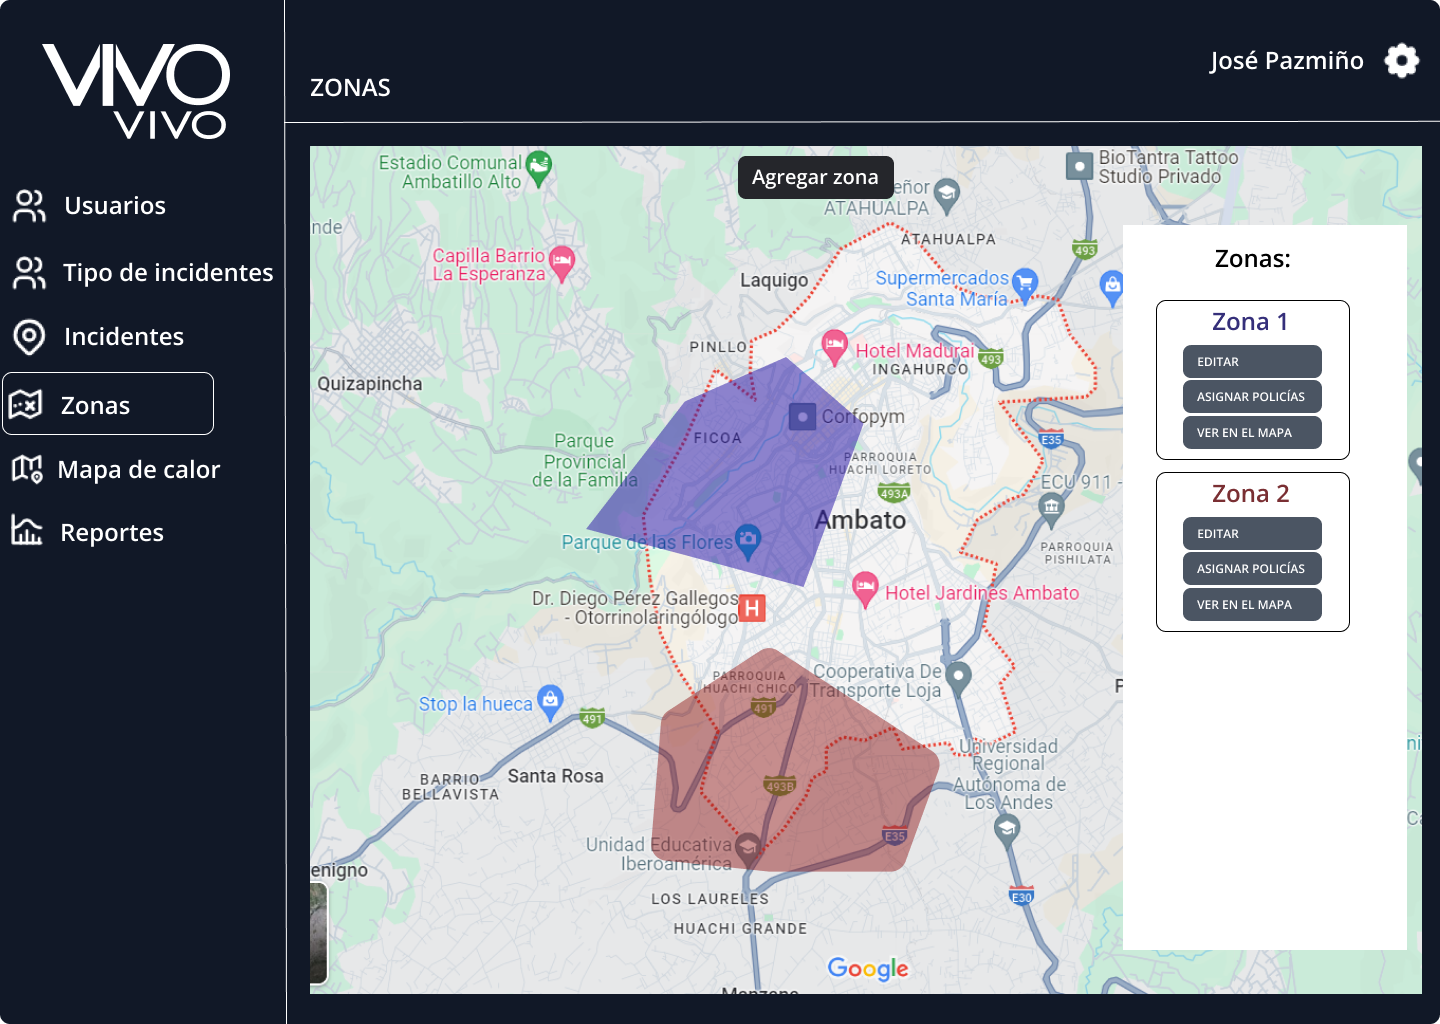
\includegraphics[width=0.6\textwidth]{chapters/III-resultados-y-discusion/resources/images/prototipo-mapa-zonas-de-vigilancia-web.png}
    \caption{Prototipo de la interfaz de usuario web: Mapa de zonas de vigilancia.}
    \label{fig:prototipo-mapa-zonas-de-vigilancia-web}
\end{figure}

Para la creación de zonas de vigilancia, se propone un formulario integrado con el mapa interactivo, el cual permite al usuario administrador
dibujar un polígono en el mapa para definir una zona de vigilancia, como se muestra en la Figura \ref{fig:prototipo-formulario-zona-vigilancia-web}.

\begin{figure}[H]
    \centering
    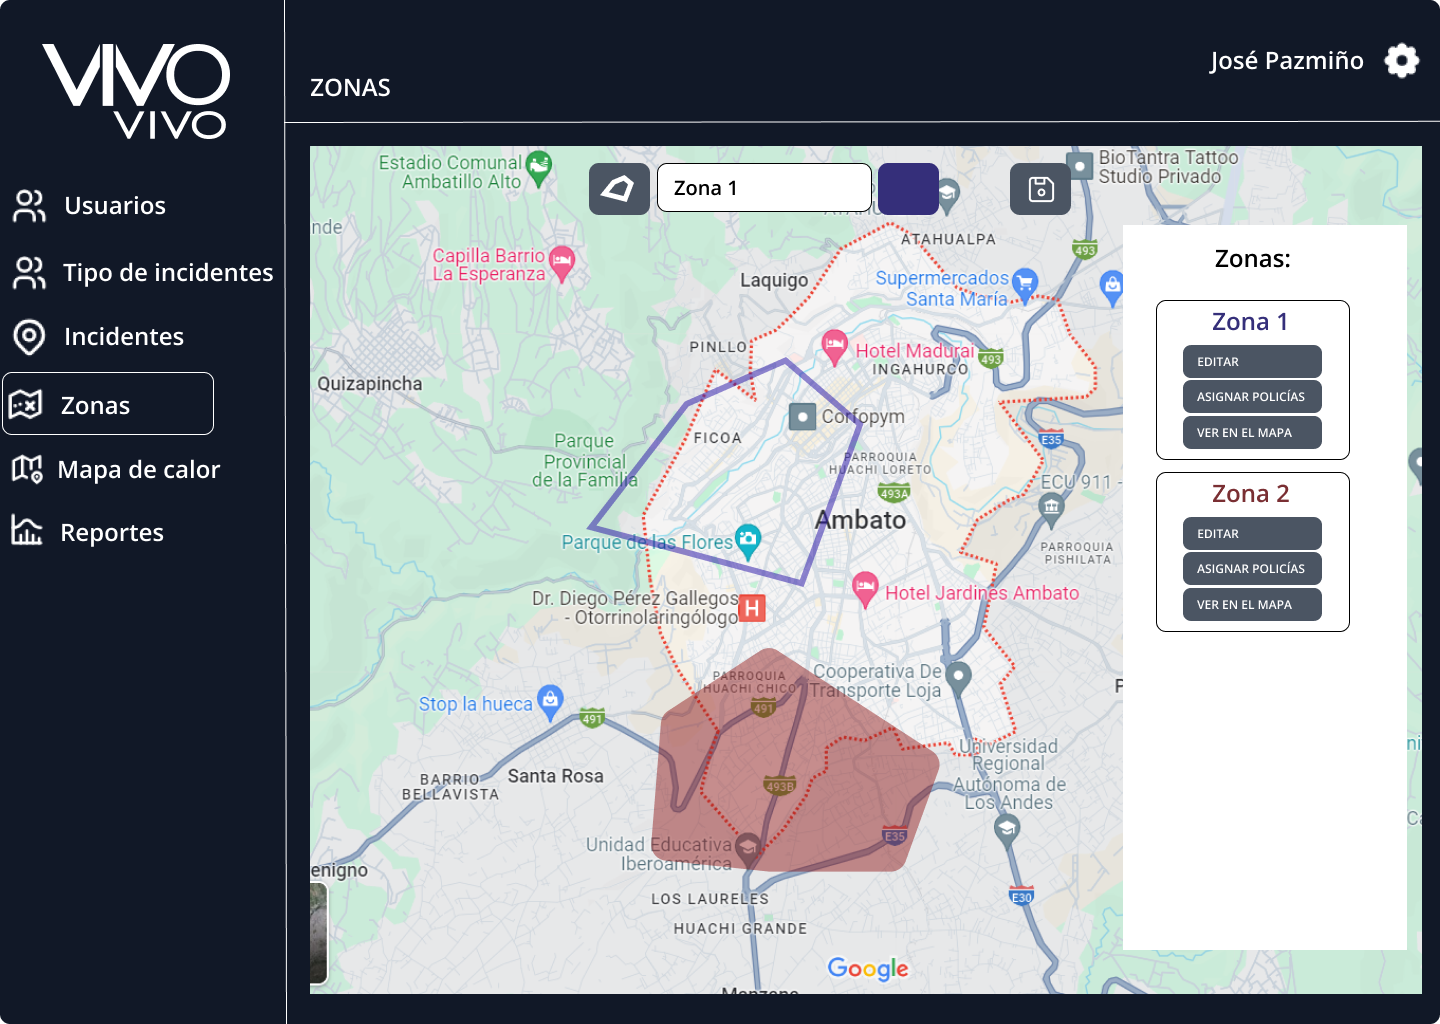
\includegraphics[width=0.6\textwidth]{chapters/III-resultados-y-discusion/resources/images/prototipo-formulario-zona-vigilancia-web.png}
    \caption{Prototipo de la interfaz de usuario web: Formulario de zona de vigilancia.}
    \label{fig:prototipo-formulario-zona-vigilancia-web}
\end{figure}

La pantalla de mapa de incidentes permite al usuario administrador visualizar los incidentes reportados en un mapa interactivo junto con la
ubicación en tiempo real de la víctima, como se muestra en la Figura \ref{fig:prototipo-mapa-incidentes-web}.

\begin{figure}[H]
    \centering
    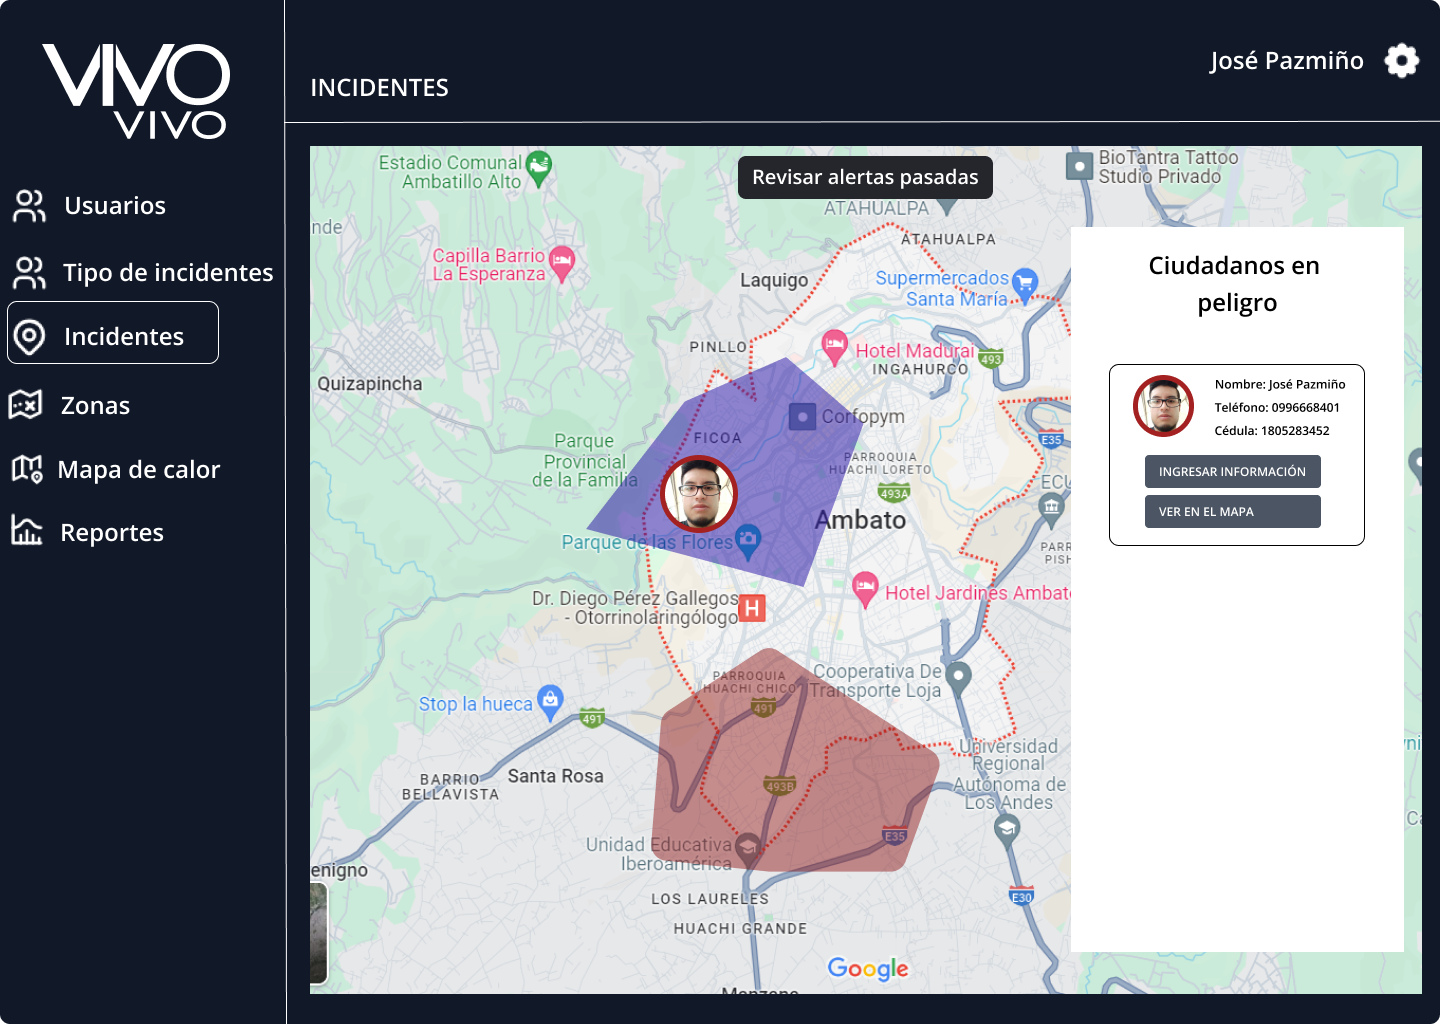
\includegraphics[width=0.6\textwidth]{chapters/III-resultados-y-discusion/resources/images/prototipo-mapa-incidentes-web.png}
    \caption{Prototipo de la interfaz de usuario web: Mapa de incidentes.}
    \label{fig:prototipo-mapa-incidentes-web}
\end{figure}

En la Figura \ref{fig:prototipo-mapa-de-calor-web} se muestra la pantalla de mapa de calor, la cual permite al usuario administrador visualizar
la densidad de incidentes reportados en un mapa interactivo mediante un gradiente de colores, así como filtrar los incidentes por tipo y fecha.

\begin{figure}[H]
    \centering
    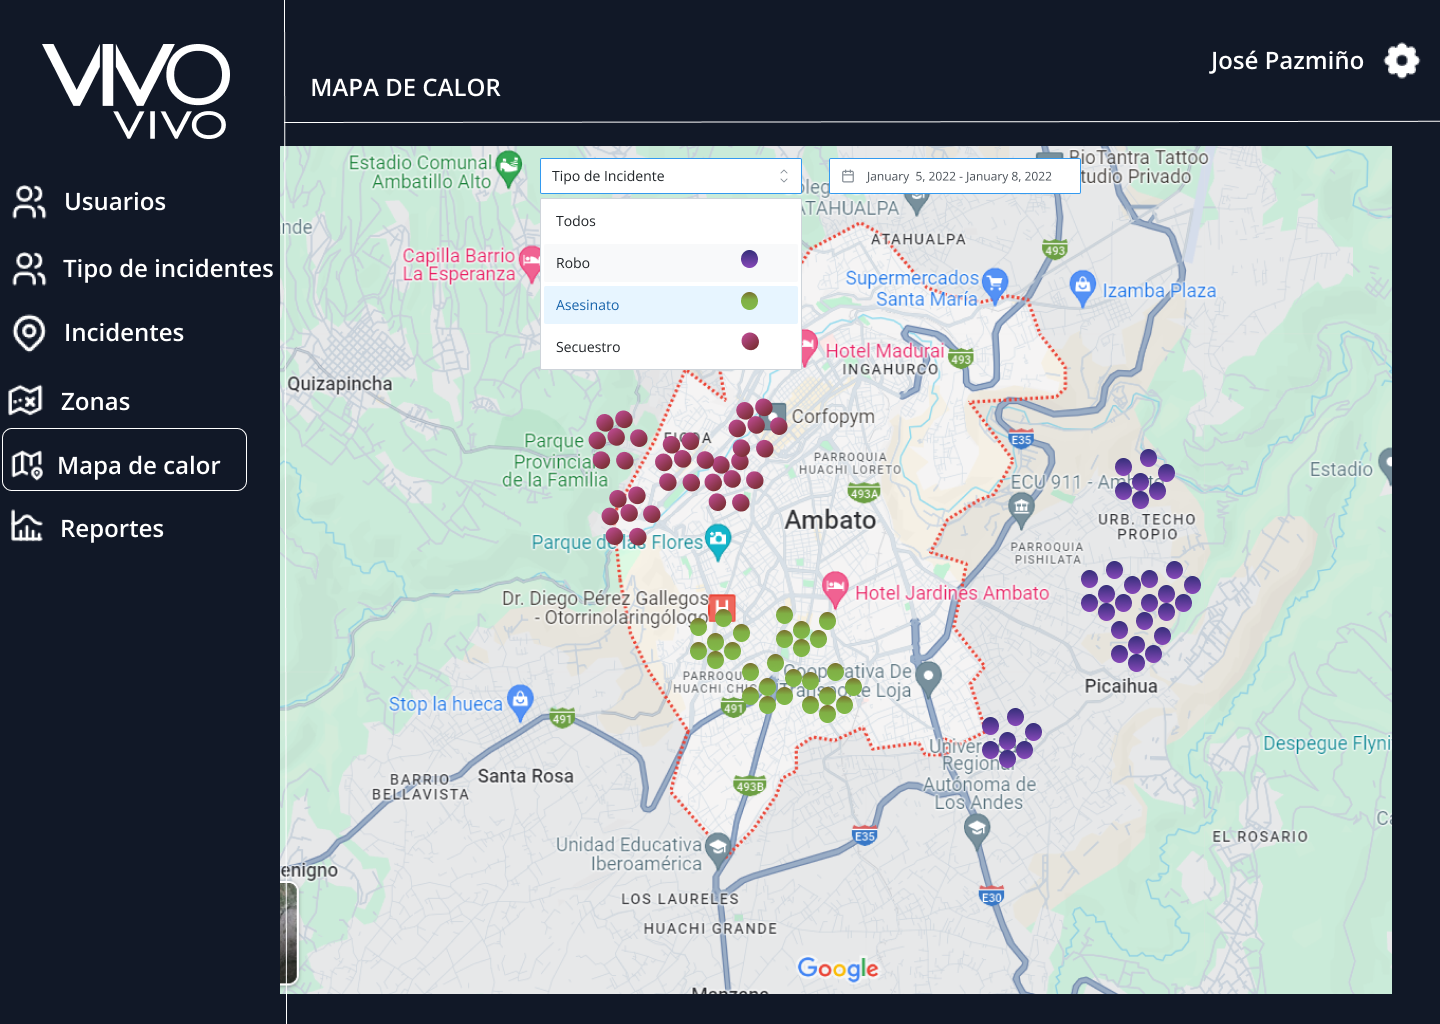
\includegraphics[width=0.6\textwidth]{chapters/III-resultados-y-discusion/resources/images/prototipo-mapa-de-calor-web.png}
    \caption{Prototipo de la interfaz de usuario web: Mapa de calor.}
    \label{fig:prototipo-mapa-de-calor-web}
\end{figure}

En la pantalla de reportería, el usuario administrador puede visualizar gráficos estadísticos de los incidentes reportados, tal como se muestra
en la Figura \ref{fig:prototipo-reporteria-web}.

\begin{figure}[H]
    \centering
    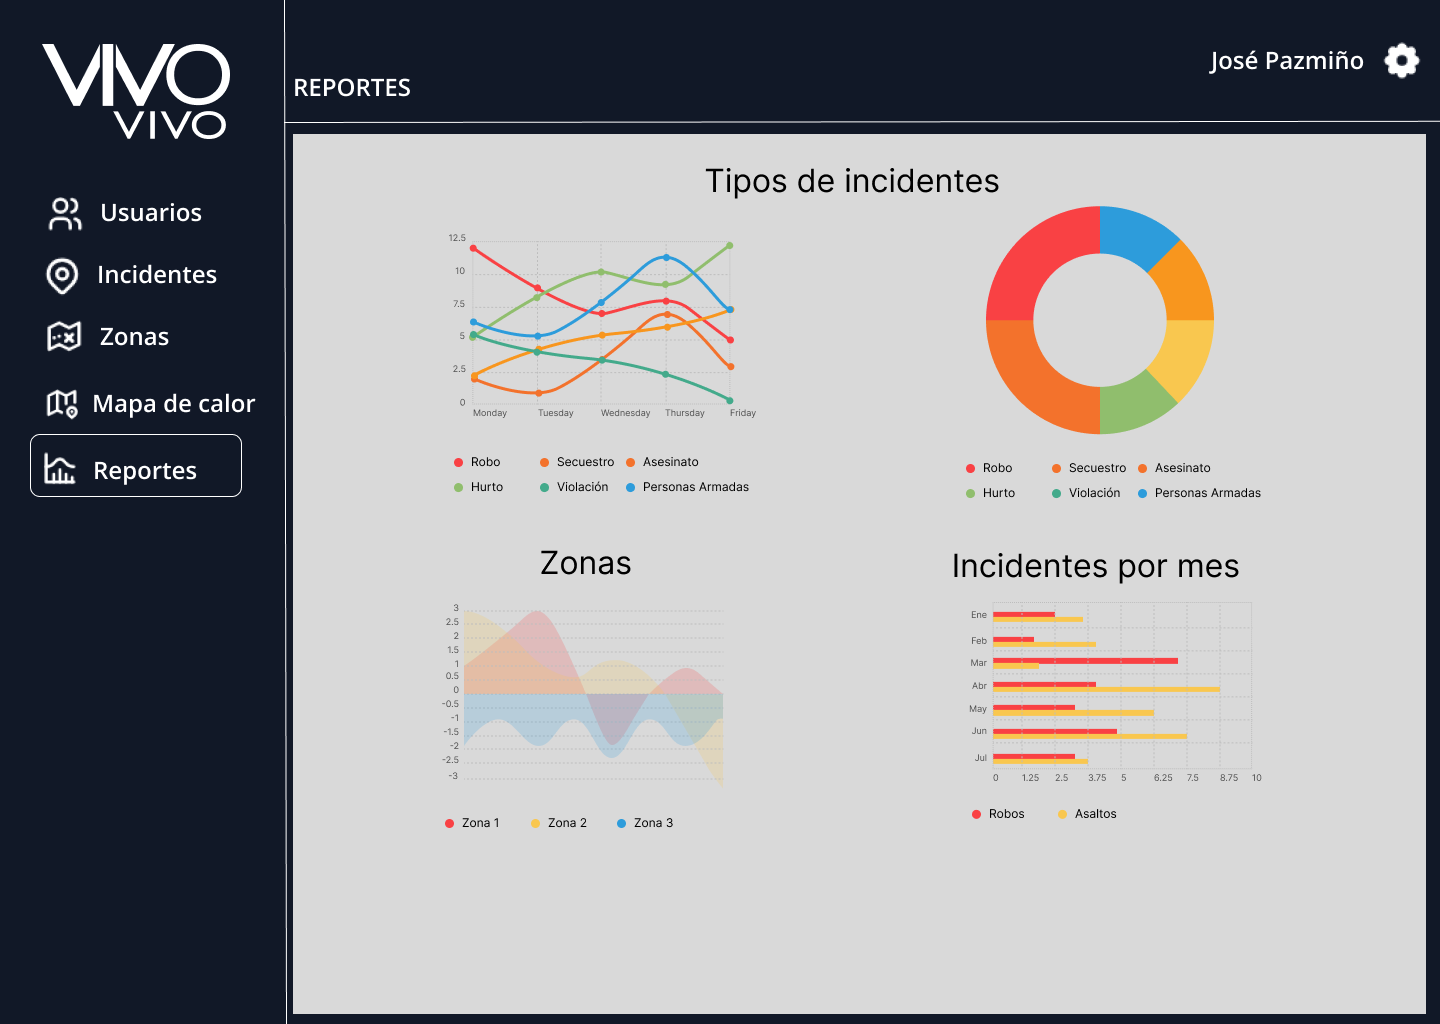
\includegraphics[width=0.6\textwidth]{chapters/III-resultados-y-discusion/resources/images/prototipo-reporteria-web.png}
    \caption{Prototipo de la interfaz de usuario web: Reportería.}
    \label{fig:prototipo-reporteria-web}
\end{figure}

\subsubsection{Prototipo de la interfaz de usuario móvil}
% TODO: REVISAR ORTOGRAFÍA
En la Figura \ref{fig:prototipo-inicio-sesion-mobile} se muestra la pantalla de inicio de sesión en la aplicación móvil, la cual se realiza mediante
el correo y contraseña del usuario.

\begin{figure}[H]
    \centering
    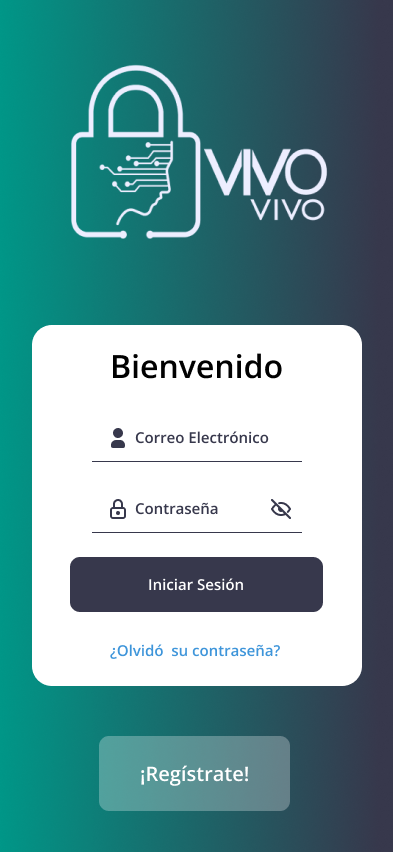
\includegraphics[width=0.3\textwidth]{chapters/III-resultados-y-discusion/resources/images/prototipo-inicio-sesion-mobile.png}
    \caption{Prototipo de la interfaz de usuario móvil: Inicio de sesión.}
    \label{fig:prototipo-inicio-sesion-mobile}
\end{figure}

Para el registro de usuarios se propone un formulario en el cual se ingresan una fotografía, nombres, apellidos, etnia, género, estado civil,
discapacidad en caso de presentarla y dirección, tal como se muestra en la Figura \ref{fig:prototipo-registro-mobile}.

\begin{figure}[H]
    \centering
    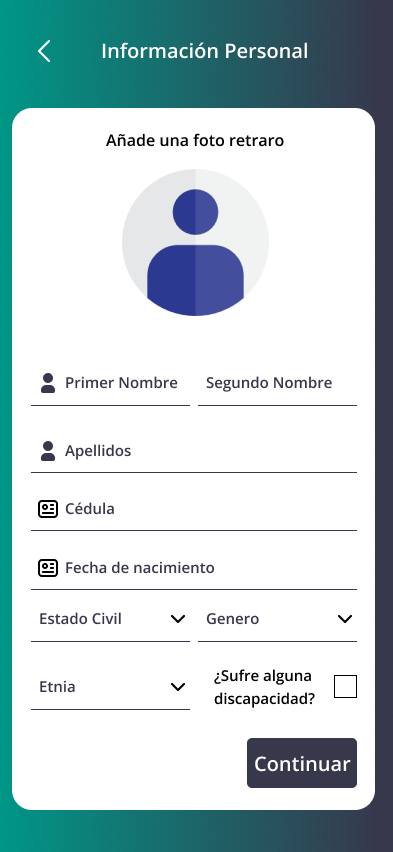
\includegraphics[width=0.3\textwidth]{chapters/III-resultados-y-discusion/resources/images/prototipo-registro-mobile.png}
    \caption{Prototipo de la interfaz de usuario móvil: Registro.}
    \label{fig:prototipo-registro-mobile}
\end{figure}

En la Figura \ref{fig:prototipo-recuperar-contrasena-mobile} se muestra la pantalla de recuperación de contraseña en la aplicación móvil, la cual se realiza
mediante el correo electrónico del usuario.

\begin{figure}[H]
    \centering
    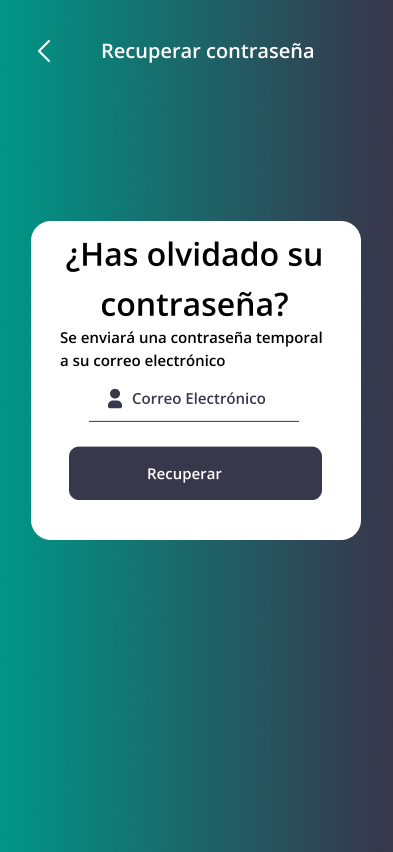
\includegraphics[width=0.3\textwidth]{chapters/III-resultados-y-discusion/resources/images/prototipo-recuperar-contrasena-mobile.png}
    \caption{Prototipo de la interfaz de usuario móvil: Recuperación de contraseña.}
    \label{fig:prototipo-recuperar-contrasena-mobile}
\end{figure}

Para la pantalla de inicio, se propone un botón de pánico que permite al usuario enviar una alerta de emergencia seleccionando el tipo de incidente y
presionando el botón durante 3 segundos para enviar la alerta. En la esquina superior derecha se encuentra el menú de opciones de la aplicación y en la
esquina superior izquierda se encuentra el botón de notificaciones de alertas de emergencia, como se muestra en la Figura \ref{fig:prototipo-inicio-mobile}.

\begin{figure}[H]
    \centering
    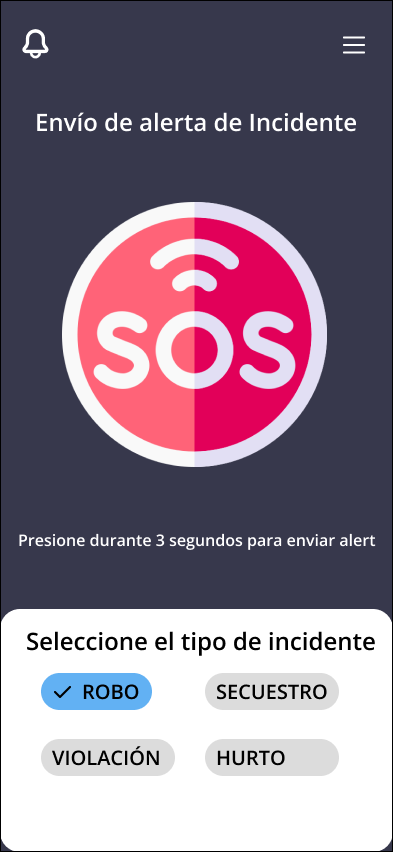
\includegraphics[width=0.3\textwidth]{chapters/III-resultados-y-discusion/resources/images/prototipo-inicio-mobile.png}
    \caption{Prototipo de la interfaz de usuario móvil: Inicio.}
    \label{fig:prototipo-inicio-mobile}
\end{figure}

En la Figura  \ref{fig:prototipo-alertas-mobile} se muestra la pantalla de alertas de emergencia, el usuario puede visualizar las alertas de emergencia
enviadas por los miembros del grupo familiar mediante una lista de alertas con la información de la persona y un botón para visualizar la ubicación
en tiempo real del incidente en un mapa interactivo como se puede observar en la Figura \ref{fig:prototipo-ubicacion-alerta-mobile}.

\begin{figure}[H]
    \centering
    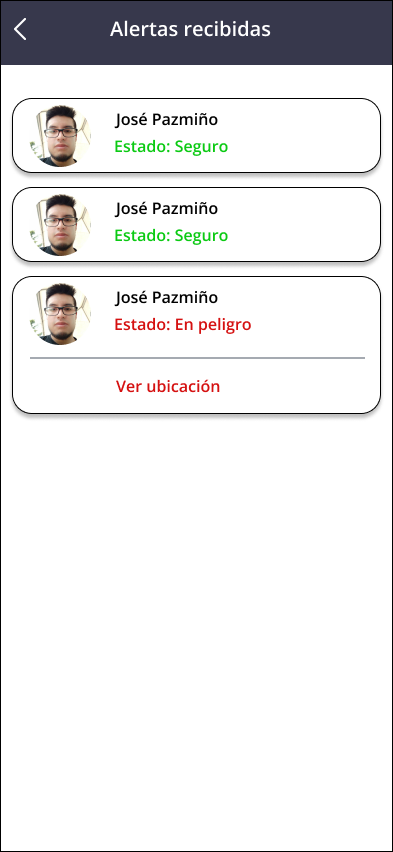
\includegraphics[width=0.3\textwidth]{chapters/III-resultados-y-discusion/resources/images/prototipo-alertas-mobile.png}
    \caption{Prototipo de la interfaz de usuario móvil: Alertas de emergencia.}
    \label{fig:prototipo-alertas-mobile}
\end{figure}

\begin{figure}[H]
    \centering
    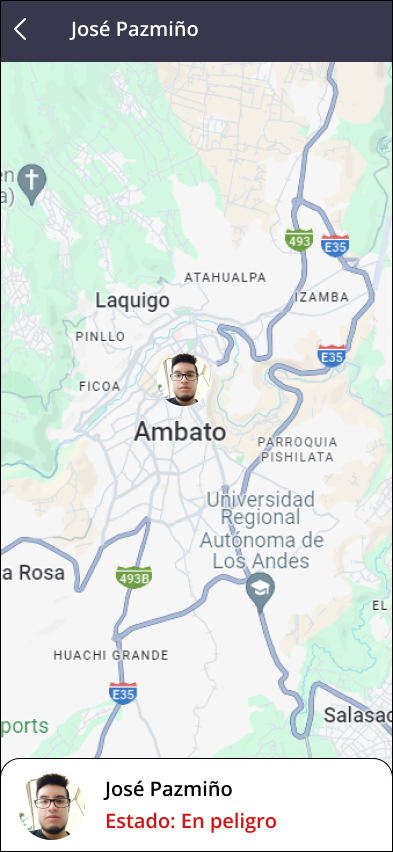
\includegraphics[width=0.3\textwidth]{chapters/III-resultados-y-discusion/resources/images/prototipo-ubicacion-alerta-mobile.png}
    \caption{Prototipo de la interfaz de usuario móvil: Ubicación de alerta.}
    \label{fig:prototipo-ubicacion-alerta-mobile}
\end{figure}

El menú de opciones de la aplicación móvil permite al usuario gestionar su grupo familiar, cambiar su contraseña y cerrar sesión, como se muestra
en la Figura \ref{fig:prototipo-menu-mobile}.

\begin{figure}[H]
    \centering
    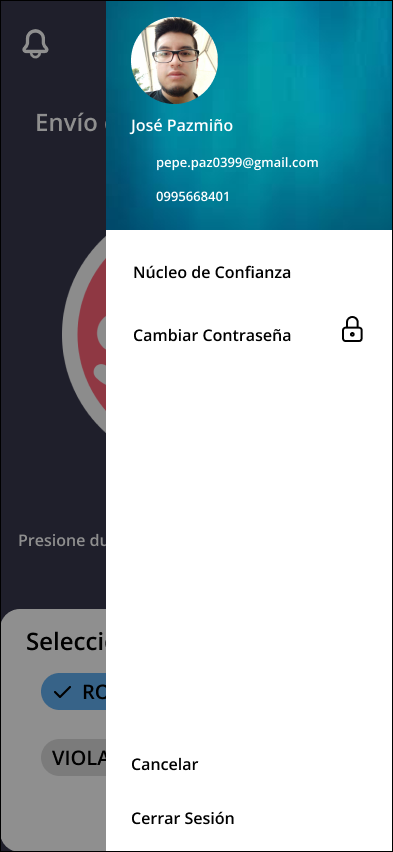
\includegraphics[width=0.3\textwidth]{chapters/III-resultados-y-discusion/resources/images/prototipo-menu-mobile.png}
    \caption{Prototipo de la interfaz de usuario móvil: Menú.}
    \label{fig:prototipo-menu-mobile}
\end{figure}

Para la gestión de grupos familiares, se propone una pantalla en la cual el usuario puede visualizar los miembros de su grupo familiar y agregar
nuevos miembros, como se muestra en la Figura \ref{fig:prototipo-grupo-familiar-mobile}. Al agregar un nuevo miembro, se muestra un formulario
en el cual se puede buscar un usuario por su cédula de identidad y agregarlo al grupo familiar, como se muestra en la Figura \ref{fig:prototipo-agregar-miembro-mobile}.

\begin{figure}[H]
    \centering
    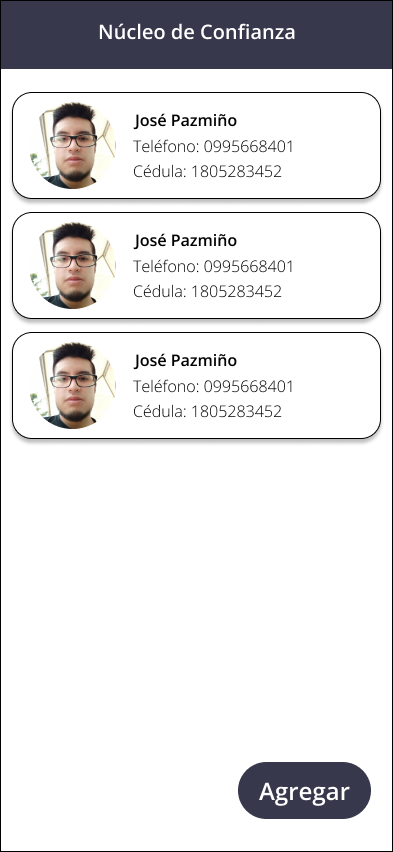
\includegraphics[width=0.3\textwidth]{chapters/III-resultados-y-discusion/resources/images/prototipo-grupo-familiar-mobile.png}
    \caption{Prototipo de la interfaz de usuario móvil: Grupo familiar.}
    \label{fig:prototipo-grupo-familiar-mobile}
\end{figure}

\begin{figure}[H]
    \centering
    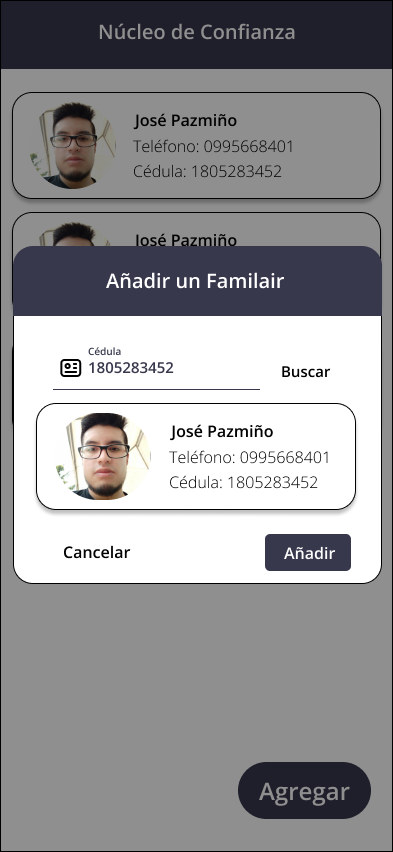
\includegraphics[width=0.3\textwidth]{chapters/III-resultados-y-discusion/resources/images/prototipo-agregar-miembro-mobile.png}
    \caption{Prototipo de la interfaz de usuario móvil: Agregar miembro.}
    \label{fig:prototipo-agregar-miembro-mobile}
\end{figure}

En la Figura \ref{fig:prototipo-cambiar-contrasena-mobile} se muestra la pantalla para cambiar la contraseña en la aplicación móvil. El usuario
debe ingresar su contraseña actual, la nueva contraseña y confirmar la nueva contraseña para realizar el cambio.

\begin{figure}[H]
    \centering
    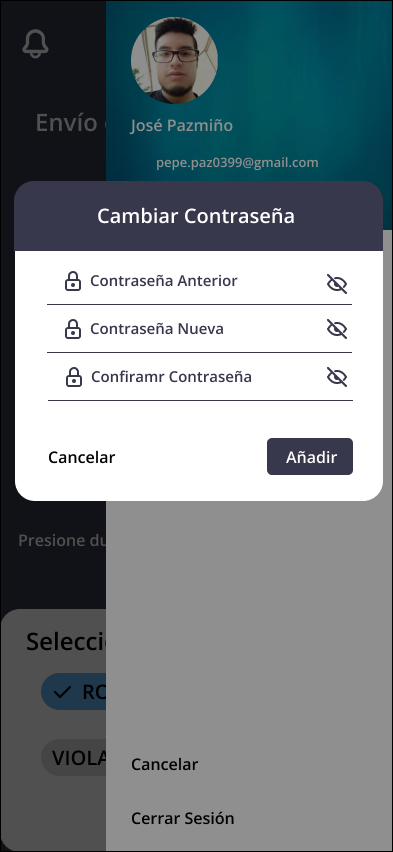
\includegraphics[width=0.3\textwidth]{chapters/III-resultados-y-discusion/resources/images/prototipo-cambiar-contrasena-mobile.png}
    \caption{Prototipo de la interfaz de usuario móvil: Cambiar contraseña.}
    \label{fig:prototipo-cambiar-contrasena-mobile}
\end{figure}
